%
% main.tex -- Paper zum Thema <maxwell>
%
% (c) 2020 Autor, OST Ostschweizer Fachhochschule
%
% !TEX root = ../../buch.tex
% !TEX encoding = UTF-8
%

\chapter{Maxwell\label{chapter:maxwell}}
\kopflinks{Maxwell-Gleichungen als Variationsprinzip}
\begin{refsection}
\chapterauthor{Maurin Doswald und Stephan Oseghale}

Als James Clerk Maxwell 1865 seine Arbeit über das elektromagnetische Feld veröffentlichte, gelang es ihm, das Wesen des elektrischen- und magnetischen Feldes, sowie die Interaktion derselben mathematisch zu beschreiben und somit das Grundwesen der Elektrodynamik aufzuzeigen.
Durch seine theoretische Arbeit konnte experimentell die Existenz von elektromagnetischen Wellen und ihre Ausbreitung mit Lichtgeschwindigkeit nachgewiesen werden.
Dies führte zu Technologien wie Radio, Radar, Fernsehen und viele weitere Anwendungen in der drahtlosen Kommunikation.

Die Grundidee zur Formulierung dieser Gleichungen kam durch eine Reihe von experimentellen Beobachtungen und theoretischen Ansätzen unterschiedlichster Wissenschaftler unter anderem Michael Faraday und André-Marie Ampère.
Durch mathematische Analysen und Experimente entwickelte Maxwell schlussendlich 20 Gleichungen, welche später von Oliver Heavyside und Willard Gibbs in die heutige bekannte vektorielle Schreibweise von vier Gleichungen gebracht wurden.
Das Ziel dieser Arbeit ist aufzuzeigen, dass die vier fundamentalen Gleichungen  auch über ein Variationsprinzip hergeleitet werden können.

%
% mathFormulierung.tex -- Felder und deren Operationen
%
% 
%
% !TEX root = ../../buch.tex
% !TEX encoding = UTF-8
%
\section{Felder\label{maxwell:mathFormulierung}}
\rhead{Felder}

Da sowohl das elektrische Feld $\vec{E}$ wie auch das magnetische Feld bzw. die magnetische Flussdichte $\vec{B}$ als Vektorfeld beschrieben werden, soll hier der Begriff des Feldes erläutert und grafisch aufgezeigt werden.

\subsection{Skalarfeld\label{maxwell:skalarfeld}}

Ein Skalarfeld ist eine Funktion der Form
\( f:\mathbb{R}^n \rightarrow \mathbb{R}, \) 
die jedem Punkt im Raum ein Skalar zuordnet.
Alltägliches Beispiele für ein Skalarfelder sind Temperaturverteilungen, Ladungsdichten oder Potentiale. In Abbildung \ref{maxwell:skalarGrad} ist das Skalarfeld einer positiven Ladung abgebildet.


%Zu den wichtigsten Operationen eines Skalarfeldes gehört der Gradient, welcher dem Skalar- ein Vektorfeld zuordnet.
%Sei $\phi$ ein Skalarfeld, dann ist $\nabla\phi$ ein Vektorfeld, dargestellt in \ref{maxwell:skalarGrad}.

\begin{figure}
	\centering
	\subfigure{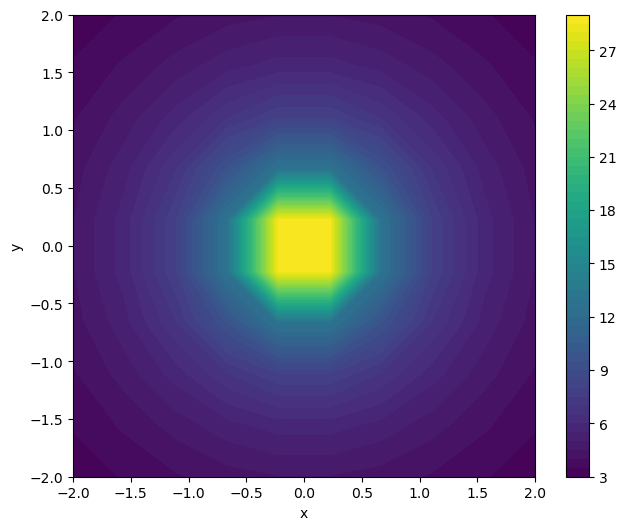
\includegraphics[width=0.35\textwidth]{papers/maxwell/skalar}}
	\subfigure{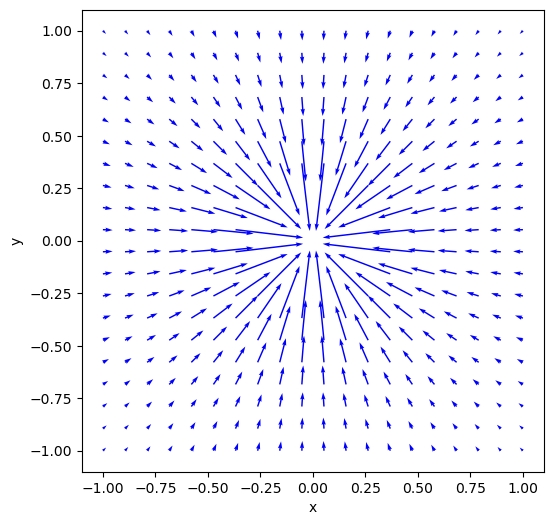
\includegraphics[width=0.3\textwidth]{papers/maxwell/gradient}}
	\caption{Skalar- und Vektorfeld}
	\label{maxwell:skalarGrad}
\end{figure}

\subsection{Vektorfeld\label{maxwell:vektorfeld}}

Ein Vektorfeld ist eine Funktion der Form \( f: \mathbb{R}^n \rightarrow \mathbb{R}^m, \) welche jedem Punkt im Raum einen Vektor zuweist. 
Die Richtung dieses Vektors gibt hierbei an, in welche Richtung der Fluss des Feldes an diesem Punkt geht, während der Betrag die Intensität repräsentiert.


Des weiteren spricht man von einem stationären Vektorfeld, wenn es zeitunabhängig ist und von einem homogenen Vektorfeld, wenn die Richtung und der Betrag der Vektoren ortsunabhängig sind, also wenn jeder Vektor die gleiche Richtung und den gleichen Betrag hat. 
Wie bereits erwähnt, sind das elektrische und das magnetische Feld, wie auch andere Kraftfelder Beispiele von Vektorfeldern.
In Abbildung \ref{maxwell:skalarGrad} ist ein Vektorfeld abgebildet.

\subsection{Operationen}

\subsubsection{Gradient}

Der Gradient wurde bereits in Abschnitt \ref{buch:fuvar:richtungsableitung:def:gradient} definiert. Dieser Operator, welcher auf ein Skalarfeld angewendet wird, resultiert in einem Vektorfeld. 
Die Richtung der Vektoren dieses neuen Vektorfeldes zeigen demnach immer in die Richtung der grössten bzw. steilsten Zunahme.
%Weiter unten wird ersichtlich, dass auch das elektrische Feld ein Gradientenfeld ist \[ \vec{E} = -\nabla\varphi, \] wobei $\varphi$ das elektrische Potential ist.

\subsubsection{Divergenz}
%TODO: Link auf Kapitel von Müller
Die Divergenz eines Vektorfeldes $\vec{F}$ ist definiert als 
\[ \text{div}\vec{F} = \nabla\cdot\vec{F} 
= \frac{\partial F_x}{\partial x} + \frac{\partial F_y}{\partial y} + \frac{\partial F_z}{\partial z}. \]
Angewendet wird sie auf ein Vektorfeld und resultiert in ein Skalarfeld.
Die Divergenz sagt aus, ob an einem Punkt mehr ``hinein-'' als ``herausfliesst'' und macht so eine Aussage über das Bestehen von Quellen und Senken. 
Wenn die Divergenz negativ ist, liegt eine Senke vor, wenn sie positiv ist eine Quelle.
Ein Vektorfeld wird quellenfrei genannt, wenn seine Divergenz zu null resultiert.

\subsubsection{Rotation}
%TODO: Link auf Kapitel von Müller
Die Rotation eines Vektorfeldes $\vec{F}$ ist definiert als
\[
\renewcommand{\arraystretch}{1.9} 
\text{rot}\vec{F} = 
\text{curl}\vec{F}
=\nabla\times\vec{F}
= \begin{pmatrix}
	\displaystyle
	\frac{\partial F_z}{\partial y} -\frac{\partial F_y}{\partial z}\\
	\displaystyle
	\frac{\partial F_x}{\partial z} -\frac{\partial F_z}{\partial x}\\
	\displaystyle
	\frac{\partial F_y}{\partial x} -\frac{\partial F_x}{\partial y}
\end{pmatrix}
. \]
Mit dieser Operation wird einem Vektorfeld ein neues Vektorfeld zugeordnet, welches eine Aussage darüber macht, wie stark das Feld sich um einen Punkt dreht bzw. rotiert.
Wenn die Rotation zu null resultiert, ist das Feld wirbelfrei.

% erste Maxwellgleichung ohne Quelle
\section{Ladungsfreie Elektrostatik
	\label{maxwell:section:equation1_ohne_quelle}}
\rhead{Problemstellung}
Man stelle sich nun einen ladungsfreien, luftleeren , drei dimensionalen Raum vor, indem ein elektrisches Potentialfeld $\phi(x,y,z)$ existiert.
Für diesen Raum möchten wir mittels der Varitaionsrechnung eine Gleichung entwickeln, die beschreibt, wie sich das Potentialfeld verhählt. 

\subsection{Ansatz}
Damit wir eine Gleichungen erhalten, die das Verhalten des elektrischen Potentialfeldes beschreibt, muss ganz allgemein die Energie im System minimiert werden. 
In diesem Fall ist die Energie im System
\[
W
=
\int_V \omega_e\, dV.
\]
Dieses Integral gilt es zu minimieren, was die Grundlage für unser Variationsproblem darstellt.
Die Energiedichte
% TODO: Bei definitionen erwähnen, dass ein vektor v^2 = v dot v ist!
\[
\omega_e\
=
\frac{1}{2}\epsilon_0\vec{E}(x,y,z)^2
\]
ist die Energiedichte im elektrischen Feld.
Diese Gleichung können wir nun mittels definition \ref{(???)} mit dem elektrischen Potentialfeld ausdrücken.
somit ist
\[
\omega_e
=
\frac{1}{2}\epsilon_0\left(-\nabla\phi(x,y,z)\right)^2.
\]
Dies können wir in das zu minimerende Integral einsetzen und bekommen
%TODO: eventuell underbraces weg lassen.
\begin{equation}
	W
	=
	\int_V \underbrace{
		\frac{1}{2}\epsilon_0\left(-\nabla\phi(x,y,z)\right)^2}_{L(x,y,z,\phi(x,y,z),\phi_x(x,y,z),\phi_y(x,y,z),\phi_z(x,y,z))}\, dV.
	\label{maxwell:section:energieintegral_quellenfrei}
\end{equation}
Aus dieser Gleichung können wir entnehmen, dass unsere Lagrangefunktion
\begin{align}
	L(x,y,z,\phi(x,y,z),\phi_x(x,y,z),\phi_y(x,y,z),\phi_z(x,y,z))
	&=
	\frac{1}{2}\epsilon_0\left(-\nabla\phi(x,y,z)\right)\cdot\left(-\nabla\phi(x,y,z)\right)
	\\
	L(x,y,z,\phi(x,y,z),\phi_x(x,y,z),\phi_y(x,y,z),\phi_z(x,y,z))
	&=
	\frac{1}{2}\epsilon_0\left(\phi_x(x,y,z)^2 + \phi_y(x,y,z)^2 + \phi_z(x,y,z)^2\right)
	\label{maxwell:section:lagrangefunktion_quellenfrei}
\end{align}
ist.
Somit haben wir unsere Lagrangefunktion gefunden, die wir in einem nächsten Schritt in die Euler-Ostrogradski-Differentialgleichung einsetzen können.

\subsection{Einsetzen in die Euler-Ostrogradski-Differentialgleichung}
%TODO: label suchen von E-O-DGL von müller kapitel
Nun gilt es die in \eqref{maxwell:section:lagrangefunktion_quellenfrei} gefundene Gleichung in die E-O-DGL \ref{???} einzusetzen.
Nach Einsetzen wird die Differentialgleichung
\[
\frac{1}{2}\epsilon_0\left(\underbrace{\frac{\partial}{\partial\phi}\left(\phi_x^2 + \phi_y^2 + \phi_z^2\right)}_{=0} - \frac{\partial}{\partial x}\frac{\partial}{\partial \phi_x}\left(\phi_x^2 + \phi_y^2 + \phi_z^2\right) - 
\frac{\partial}{\partial y}\frac{\partial}{\partial \phi_y}\left(\phi_x^2 + \phi_y^2 + \phi_z^2\right) - 
\frac{\partial}{\partial z}\frac{\partial}{\partial \phi_z}\left(\phi_x^2 + \phi_y^2 + \phi_z^2\right)\right)
=
0.
\]
Man sieht, dass die partielle Ableitung nach $\phi$ verschwindet.
Nach den partiellen Ableitungen nach $\phi_x$, $\phi_y$ und $\phi_z$ wird die Differentialgleichung
\[
\frac{1}{2}\epsilon_0\left(-\frac{\partial}{\partial x}2\phi_x(x,y,z) - \frac{\partial}{\partial y}2\phi_y(x,y,z) - \frac{\partial}{\partial z}2\phi_z(x,y,z)\right)
=
0.
\]
Wenn man nun noch die letzten partiellen Ableitungen macht, wird die Differentialgleichung
\begin{equation}
	- \underbrace{\epsilon_0}_{\not{=}0}\underbrace{\left(\frac{\partial^2\phi(x,y,z)}{\partial x^2} + \frac{\partial^2\phi(x,y,z)}{\partial y^2} + \frac{\partial^2\phi(x,y,z)}{\partial z^2}\right)}_{=0}
	=
	0.
	\label{maxwell:section:laplace_gleichung_1}
\end{equation}
%definiton des laplace operators suchen
An dieser Gleichung sieht man, dass die Klammer mit den partiellen Ableitungen gleich null sein muss, da die Permittivität von Vakuum nicht null sein kann.
Zusätzlich wird nun ersichtlich, dass der Klammerterm nach definition \ref{???} mit dem Laplace-Operator angewendet auf das elektrische Potentialfeld $\phi$ ersetzt werden kann.
Somit wird unsere schluss Differentialgleichung
\begin{equation}
	\Delta\phi(x,y,z)
	=
	0.
	\label{maxwell:section:laplace_gleichung_2}
\end{equation}
Durch Anwendng der Definiton des Laplace-Operator \ref{???} und der Definiton des Elektrischenfeldes \ref{???} erhalten wird die Gleichung
\[
\nabla\cdot\underbrace{\nabla\phi(x,y,z)}_{-\vec{E}(x,y,z)}
=
0.
\]
Hiermit erhalten wir, dass
\begin{equation}
	\nabla\cdot\vec{E}(x,y,z)
	=
	0
	\label{maxwell:section:e_feld_quellenfrei}
\end{equation}
% TODO:Bild referenz einfügen und Bild erstellen
sein muss. Diese Differentialgleichung besagt, dass das Elektrische Feld quellenfrei ist.
Dies bedeutet, dass Felldlinien des Elektrischenfeldes an keinem Ort im Raum enstehen oder enden können \ref{???}.
Dies ist sehr naheliegend, da ohne Ladungen im Raum das Elektrische Feld quellenfrei sein muss.

\subsubsection{Exkurs zur Laplace-Gleichung}
Potentialfelder, die die Laplace-Gleichung
\[
\Delta\varphi
=
0
\]
erfüllen, 





%
% einleitung.tex -- Beispiel-File für die Einleitung
%
% (c) 2020 Prof Dr Andreas Müller, Hochschule Rapperswil
%
% !TEX root = ../../buch.tex
% !TEX encoding = UTF-8
%
%erste Maxwell Gleichung mit Quelle
\subsection{Gausssches Gesetz des elektrischen Feldes
\label{maxwell:section:elektrostatik_mit_quelle}}
Nun betrachten wir einen luftleeren, dreidimensionalen Raum $V\subset\mathbb{R}^3$, in dem ein elektrisches Potentialfeld $\varphi(x,y,z)$ und eine Ladungsdichte $\varrho(x,y,z)$ existieren.
Auch für diesen Raum möchten wir mittels der Variationsrechnung eine partielle Differentialgleichung finden, die das Verhalten des elektrischen Potentialfeldes beschreibt.

\subsubsection{Ansatz}
Es ist naheliegend, dass auch in diesem Szenario die Energie im System minimiert werden muss.
Wie auch in Gleichung \eqref{maxwell:section:energieintegral_quellenfrei} ist die Energie im elektrischen Feld
\[
W_{\text{e}}
=
\iiint_V \frac{1}{2}\,\varepsilon_0\,(\varphi_x^2 + \varphi_y^2 + \varphi_z^2)\, dV.
\]
Jedoch ist dies nicht die einzige Komponente der Gesamtenergie des Systems.
Laut \eqref{maxwell:section:definition_elektrischespotentialfeld} ist das elektrische Potential eine auf die Ladung normierte potentielle Energie.
Somit haben wir die fehlende Komponente gefunden.
Damit wir die durch die Ladung
\begin{equation}
q
=
\iiint_V \varrho(x,y,z)\, dV
\label{maxwell:ladung}
\end{equation}
verursachte potentielle Energie $W_{\text{q}}$ im System mit der Ladungsdichte $\varrho$ ausdrücken können, müssen wir untersuchen, was eine infinitesimale potentielle Energie verursacht.
Wenn wir diese infinitesimal kleine potentielle Energie
\(
dW_{\text{q}}
=
\varphi\, dq
\)
unter die Lupe nehmen und für die infinitesimal kleine Ladung
\(
dq
=
\varrho\, dV
\)
einsetzen, erhalten wir
\(
dW_{\text{q}}
=
\varphi\,\varrho\, dV.
\)
Jetzt müssen die infinitesimalen potentiellen Energien im Raum $V$ zusammengezählt werden und es resultiert
\begin{equation}
W_{\text{q}}
=
\iiint_V \varphi\,\varrho\, dV.
\label{maxwell:section:potenzielle_energie_ladung}
\end{equation}
Mit der Gesamtenergie
\[
W_{\text{tot}}
=
W_{\text{e}} - W_{\text{q}}
=
\iiint_V \frac{1}{2}\,\varepsilon_0\left(\varphi_x^2 + \varphi_y^2 + \varphi_z^2\right) - \varphi\,\varrho\, dV
\]
des Systems haben wir unser zu minimierendes Integral gefunden.
Daraus können wir wieder die Lagrange-Funktion
\begin{equation}
L(x,y,z,\varphi,\varphi_x,\varphi_y,\varphi_z)
=
\frac{1}{2}\,\varepsilon_0\left(\varphi_x^2 + \varphi_y^2 + \varphi_z^2\right) - \varphi\,\varrho
\label{maxwell:section:lagrangefunktion_mit_quelle}
\end{equation}
% TODO: Müller fragen wegen kopplungsterme
ablesen.
Man bemerkt, dass die Lagrange-Funktion einen zusätzlichen additiven Term erhalten hat im Verlgeich zur Lagrange-Funktion \eqref{maxwell:section:lagrangefunktion_quellenfrei}.
Solche Terme nennt man Kopplungsterme.
Sie werden verwendet, um die Wechselwirkung zwischen Termen in der La\-gran\-ge-Funktion zu berücksichtigen.
Der Kopplungsterm in unserem Fall beschreibt die Wechselwirkung zwischen dem Feld und der Ladungsdichte.
Nun können wir diese Lagrange-Funktion in die Euler-Ostrogradski-Differentialgleichung einsetzen, um zu untersuchen, wie sich das elektrische Potentialfeld verhält.

\subsubsection{Einsetzen in die Euler-Ostrogradski-Differentialgleichung}
Jetzt wollen wir, die in \eqref{maxwell:section:lagrangefunktion_mit_quelle} gefundene Lagrange-Funktion in die Euler-Ostrogradski-Differentialgleichung einsetzten.
Um die Rechnung übersichtlicher zu gestalten, machen wir uns die Linearität der Euler-Ostrogradski-Differentialgleichung
\begin{equation}
F(W_{\text{tot}})
=
F(W_{\text{e}} - W_{\text{q}})
=
F(W_{\text{e}}) + F(-W_{\text{q}})
\label{maxwell:section:linearität_von_DGL}
\end{equation}
zu nutze.
Die Lösung von $F(W_{\text{e}})$ haben wir in Gleichung \eqref{maxwell:section:laplace_gleichung_1} bereits gefunden.
Durch einsetzen von $-W_{\text{q}}$ in die Euler-Ostrogradski-Differentialgleichung erhalten wir
\[
\frac{\partial}{\partial\varphi}\left(-\varrho\,\varphi\right) - \frac{\partial}{\partial x} \underbrace{\frac{\partial}{\partial\varphi_x}\left(\varrho\,\varphi\right)}_{\displaystyle=0} - \frac{\partial}{\partial y} \underbrace{\frac{\partial}{\partial\varphi_y}\left(\varrho\,\varphi\right)}_{\displaystyle=0} - \frac{\partial}{\partial z} \underbrace{\frac{\partial}{\partial\varphi_z}\left(\varrho\,\varphi\right)}_{\displaystyle=0}
=
0.
\]
Da alle partiellen Ableitungen nach $\varphi_x, \varphi_y, \varphi_z$ null ergeben, müssen wir nur noch die partielle Ableitung nach $\varphi$ durchführen.
Somit ist
\(
-\varrho
=
0.
\)
Durch Addition unserer zwei Teillösungen erhalten wir die Gleichung
\begin{align*}
-\varepsilon_0\,\Delta\varphi - \varrho
&=
0
\\
\Leftrightarrow \qquad \varepsilon_0\,\Delta\varphi
&=
-\varrho.
\end{align*}
Schlussendlich ist
\begin{equation}
\Delta\varphi
=
-\frac{\varrho}{\varepsilon_0}.
\label{maxwell:section:erste_maxwellgleichung_1}
\end{equation}
% TODO: definiton des laplace-operators suchen
Durch gleiches Vorgehen wie in Gleichung \eqref{maxwell:section:laplace_gleichung_3} erreichen wir, dass
\[
\nabla\cdot\underbrace{\nabla\varphi}_{\displaystyle-\vec{E}}
=
-\frac{\varrho}{\varepsilon_0}
\]
ist.
Somit können wir erneut die Schlussdifferentialgleichung mit dem elektrischen Feld ausdrücken.
Dadurch muss
\begin{equation}
\nabla\cdot\vec{E}
=
\frac{\varrho}{\varepsilon_0}
\label{maxwell:section:erste_maxwellgleichung_2}
\end{equation}
gelten.
Wir sehen, dass dies dem gaussschen Gesetz des elektrischen Feldes entspricht.
\index{Gesetz von Gauss}%

\subsubsection{Interpretation des Resultates}
Das gausssche Gesetz \eqref{maxwell:section:erste_maxwellgleichung_2} besagt, dass die Quelle des elektrischen Feldes eine Ladungsdichte $\varrho$ ist.
Dies bedeutet, dass elektrische Feldlinien auf Ladungen enden können.
In anderen Worten wird das elektrostatische Feld durch Ladungen erzeugt!
Da es sowohl positive wie auch negative Ladungen gibt, existieren demnach auch positive und negative Ladungsdichten.
Wenn die Ladungsdichte positiv ist, sagt uns das gausssche Gesetz, dass das elektrische Feld eine Quelle besitzt.
Das heisst, salopp gesagt, die Feldvektoren zeigen weg von der Ladungsdichte.
Wenn die Ladungsdichte jedoch negativ ist, besitzt das elektrische Feld eine Senke.
Das heisst in diesem Fall, dass die Feldvektoren auf die Ladungsdichte zeigen. Dies ist in Abbildung \ref{maxwell:section:E-Feld_punktladung} veranschaulicht.

\subsubsection{Exkurs zur Poisson-Gleichung}
\index{Poisson-Gleichung}%
% Darf auch weggelassen werden.
Die Poisson-Gleichung
\[
\Delta\varphi
=
f,
\]
wobei $\varphi$ ein Potentialfeld und $f$ eine Quelle ist, findet in vielen Teilen der Physik ihre Anwendungen.
Die Quelle $f$ kann wie in Gleichung \eqref{maxwell:section:erste_maxwellgleichung_1} eine Funktion des Raumes und/oder eine Funktion der Zeit sein.
Ein Potentialfeld, dass die Poisson-Gleichung erfüllt, führt zu einem Gradientenfeld $\nabla\varphi$, dass die Quelle $f$ besitzt und rotationsfrei ist.
Die homogene Gleichung, also jene die $f = 0$ erfüllt, führt uns zur Laplace-Gleichung.








%
% magnetostatik.tex -- Herleitung Amperesches Gesetz über E-O-DGL
%
% (c) 2020 Prof Dr Andreas Müller, Hochschule Rapperswil
%
% !TEX root = ../../buch.tex
% !TEX encoding = UTF-8
%
\section{Magnetostatik\label{maxwell:magnetostatik}}
\rhead{Magnetostatik}


Wenn sich eine Ladung mit konstanter Geschwindigkeit bewegt, entsteht um sie herum ein rotationssymmetrisches Magnetfeld. Darüber hinaus wirken auch magnetische Kräfte auf die Ladung.
Wenn sich viele Ladungen mit einer konstanten Geschwindigkeit durch einen Leiter bewegen, erzeugen diese einen konstanten Strom, welcher ein konstantes magnetisches Feld, also ein Feld, welches sich über die Zeit nicht ändert, zur Folge hat. Dieses wirkt konzentrisch um den Leiter, wie in Abbildung \ref{maxwell:flussdichte} ersichtlich ist. Ausserdem ist in der Abbildung ersichtlich, dass die Feldlinien einen geschlossenen Pfad bilden. Dies zeigt, dass das magnetische Feld keine Quellen aufweist, also quellenfrei ist, und dass es somit keine magnetischen Monopole gibt.

In der Magnetostatik betrachten wir also stationäre magnetische Felder, die Ursache dafür sind Permanentmagnete oder wie bereits erwähnt Gleichströme bzw. Ladungen mit konstanter Geschwindigkeit.
Wir setzen also neu
\[ 
\frac{\partial q}{\partial t}
=
I
=
\text{const}
\]
voraus.
Zusätzlich konzentrieren wir uns in diesem Abschnitt ausschliesslich auf das magnetische Feld bzw. die magnetische Flussdichte, also nur magnetische Phänomene, somit wird auch
\[\varphi(x,y,z) = 0 \qquad \forall x,y,z\, ,\] 
also das elektrische Potentialfeld im gesamten Raum als null angenommen. 



\begin{figure}
\centering
% WIRE B FIELD 3D
\begin{tikzpicture}[z={(0.8,0.28)},x={(0.58,-0.45)}]
	
	\def\L{6}
	\def\W{0.10}
	\def\R{0.9}
	\def\ang{-35}
	\def\scale{1.3}
	\def\NB{5}
	\coordinate (O) at (0,0,0);
	%\draw (0,0,0) -- (2,0,0);
	%\draw (0,0,0) -- (0,0,2);
	
	% Koordinatensystem
	\draw[->] (0,0,0) -- (3,0,0) node[anchor=north east]{$x$};
	\draw[->] (0,0,0) -- (0,3,0) node[anchor=north west]{$z$};
	\draw[->] (0,0,0) -- (0,0,4) node[anchor=south]{$y$};
	
	% B FIELD BACK
	\foreach \i [evaluate={\x=(\i-\NB/2-0.5)*\L/\NB;}] in {1,...,\NB}{
		%\draw[BField,-] (0,0,\x)++(\ang+1:\R) arc (\ang+1:\ang-181:\R);
		\draw[BFieldLine=1] (0,0,\x)++(\ang+1:\R) arc (\ang+1:\ang-181:\R) --++ (65:0.001*\R);
	}
	
	% WIRE
	\draw[metal] (0,0,-\L/2)++(120:\W/2) --++ (0,0,\L) arc (120:-60:\W/2) --++ (0,0,-\L) arc (-60:120:\W/2);
	\draw[metal] (0,0,-\L/2) circle (\W/2);
	\draw[current] (0.12*\R,-0.12*\R,0.4*\L) --++ (0,0,0.2*\L) node[below=2,right] {$I$};
	
	% B FIELD FRONT
	\foreach \i [evaluate={\x=(\i-\NB/2-0.5)*\L/\NB;}] in {1,...,\NB}{
		%\draw[BFieldLine=1] (0,0,\x)++(\ang+180:\R) arc (\ang+180:\ang:\R) --++ (-116:0.001*\R);
		\draw[BField,-] (0,0,\x)++(\ang+180:\R) arc (\ang+180:\ang:\R);
	}
	\node[Bcol] at (-0.9*\R,0.9*\R,-0.25*\L) {$\vec{B}$}; %++(140:1.3*\R)
	
\end{tikzpicture}
	\caption{Magnetische Flussdichte um einen geraden Leiter}
	\label{maxwell:flussdichte}
\end{figure}




\subsubsection{Magnetisches Vektorpotential}

Wie auch in der Elektrostatik, gibt es in der Magnetostatik ein Potential, mit welchem energetische Zustände berechnet und ausgedrückt werden können. Im Unterschied ist jedoch das magnetische Potential ebenfalls eine vektorielle Grösse, also auch ein Vektorfeld. Das magnetische Vektorpotential zeigt jeweils in die selbe Richtung wie der Geschwindigkeitsvektor der bewegten Ladung.
Durch das magnetische Vektorpotential, kann die magnetische Flussdichte als 
\begin{equation}
	\operatorname{rot}\vec{A}=\nabla \times \vec{A}
	=
	\vec{B}
	\label{maxwell:definitionVektorpot}
\end{equation}
beschrieben werden, wobei wir dies für später bereits konkret ausrechnen wollen 
\begin{equation}
	\label{maxwell:nablaA}
	\renewcommand{\arraystretch}{1.9}
	\begin{pmatrix}
		\displaystyle
		\frac{\partial}{\partial x} \\
		\displaystyle
		\frac{\partial}{\partial y} \\
		\displaystyle
		\frac{\partial}{\partial z}
	\end{pmatrix}
	\times
	\begin{pmatrix}
		\displaystyle
		A_1 \\
		A_2 \\
		A_3 \\
	\end{pmatrix}
	=
	\begin{pmatrix}
		\displaystyle
		\frac{\partial A_3}{\partial y} -\frac{\partial A_2}{\partial z}\\
		\displaystyle
		\frac{\partial A_1}{\partial z} -\frac{\partial A_3}{\partial x}\\
		\displaystyle
		\frac{\partial A_2}{\partial x} -\frac{\partial A_1}{\partial y}
	\end{pmatrix}.
\end{equation}
Im Gegensatz zum elektrischen Feld, ist das magnetische Feld also kein Gradientenfeld seines Potentials, sondern ein Rotationsfeld.

Analog zur Elektrostatik, lässt sich mit dem magnetischen Vektorpotential die potentielle Energie der Wirkgrösse berechnen. Die Wirkgrösse ist jetzt allerdings keine ruhende Ladung $q$ mehr, sondern eine Ladung $q$ mit einer Geschwindigkeit $\vec{v}$, also eine bewegte Ladung. Explizit lässt sich die potentielle Energie als 
\[ W_{\text{p}} =  q\vec{v}\cdot\vec{A}\]
berechnen. Also das Skalarprodukt der Wirkgrösse und dem Potential des wirkenden Feldes an jenem Punkt im Raum.


%Mit dem Vektorpotential können ähnlich wie beim elektrischen Potential, energetische Zustände beschrieben werden. Die Wirkgrösse hier ist allerdings eine bewegte Ladung also eine Ladung $q$, welche eine Geschwindigkeit $\vec{v}$ hat. So kann das magnetische Potential dieser Grösse an einem Punkt berechnet werden. Zusätzlich ergibt sich über das Vektorpotential so auch die potentielle Energie dieser Wirkgrösse, auf welche weiter unten noch spezifischer eingegangen wird.


\subsection{Ampèresches Gesetz}
Das Ziel dieses Abschnitts ist erneut eine partielle Differentialgleichung zu finden, welche das Wesen des magnetischen Vektorpotentials und somit des magnetischen Feldes beschreibt.
Wiederum betrachten wir unter den oben vorausgesetzten Bedingungen einen luftleeren, dreidimensionalen Raum $V \subset \mathbb{R}^3$ in welchem das Vektorfeld des magnetischen Vektorpotentials $\vec{A}(x,y,z)$, somit das magnetische Feld $\vec{B}(x,y,z)$ und eine magnetische Wirkgrösse $q\vec{v}$  existieren. 

\subsubsection{Ansatz}

Wieder soll die Energie des gesamten Systems zusammengetragen und minimiert werden. 
Die Energiedichte des magnetischen Feldes mit \eqref{maxwell:definitionVektorpot} eingesetzt ist
\[ w_{\text{m}} 
= 
\frac{1}{2\mu_0}\vec{B}(x,y,z)^2
=
\frac{1}{2\mu_0}\left(\nabla\times\vec{A}(x,y,z)\right)^2. \]
Die Gesamtenergie jenes berechnet sich dadurch als
\begin{equation}
	\label{maxwell:magnetFeldEnergie}
	W_{\text{m}} = \iiint_V w_m\, dV\,.
\end{equation}
Wie bereits erwähnt, ergibt sich durch eine bewegte Ladung $q$ mit einer Geschwindigkeit $\vec{v}$ eine weitere potentielle Energie im System, welche sich als 
\[ 
W_{\text{p}}
= 
q\vec{v}
\cdot
\vec{A}
 \]
berechnen lässt.
Da unser Ziel jedoch ist, das Integral der Gesamtenergie zu minimieren, müssen wir auch diese potentielle Energie über den gesamten Raum bzw. das selbe Volumen integrieren wie das Integral in \eqref{maxwell:magnetFeldEnergie}. 

Dafür betrachten wir erneut nur ein kleines, ein infinitesimales Stück der Ladung also $dq\,\vec{v}$ und können mithilfe von $dq = \varrho\,dV$, wobei $\varrho$ die Ladungsdichte ist, dieses kleine Stück der Ladung sofort zu $\vec{v}\varrho\,dV$ umschreiben.
Wenn wir uns jetzt überlegen, dass sich eine Ladungsdichte mit einer Geschwindigkeit $\vec{v}$ bewegt, können wir auch sagen, dass dies äquivalent zu einer Stromdichte $\vec{\jmath}=\varrho\vec{v}$ ist. 
Die kleinen bzw. infinitesimalen Stücke der Wirkgrösse formen wir also zu \[\vec{\jmath}\,dV = \varrho\vec{v}\,dV\]
um und erhalten mit einer Integration über den ganzen Raum $V$
\begin{equation}
	W_{\text{p}}
	= 
	\iiint_V \vec{A}\cdot\varrho\vec{v}\,dV
	=
	\iiint_V \vec{A}(x,y,z)\cdot\vec{j}(x,y,z)\,dV
\end{equation}
die gesamte potentielle Energie der Wirkgrösse.

Jetzt befinden sich beide Energiekomponenten in einer Form, in welcher wir über denselben Raum bzw. dasselbe Volumen integrieren können und somit lassen sie sich zu einem einzigen Integral als 
\begin{align*}
W_{\text{tot}} 
&=
W_{\text{p}} - W_{\text{m}}
=
\iiint_V \vec{A}\cdot\vec{\jmath}
- \frac{1}{2\mu_0}\left(\nabla\times\vec{A}\right)\cdot\left(\nabla\times\vec{A}\right)\, dV \\
&=
\iiint_V \left( A_1j_1 + A_2j_2 + A_3j_3\right) - 
 \frac{1}{2\mu_0}\biggl( 
 	\left( \frac{\partial A_3}{\partial y} -\frac{\partial A_2}{\partial z}\right)^2 
 + \left( \frac{\partial A_1}{\partial z} -\frac{\partial A_3}{\partial x}\right)^2
 + \left(\frac{\partial A_2}{\partial x} -\frac{\partial A_1}{\partial y} \right)^2   
 \biggr) \,dV
\end{align*}
zusammenfassen.

In dieser Gleichung wird sofort das zu minimierende Integral ersichtlich und die Lagrange-Funktion kann als 

	%\begin{align}
	%\label{maxwell:magnetostatikLagrange}
	%L\left(x,y,z, \vec{A}, \vec{A}_x. \vec{A}_y, \vec{A}_z\right)
	%=&\left( A_1j_1 + A_2j_2 + A_3j_3\right) \\ \nonumber
	% &- \frac{1}{2\mu_0}\left( 
	%\left( \frac{\partial A_3}{\partial y} -\frac{\partial A_2}{\partial %z}\right)^2 
	%+ \left( \frac{\partial A_1}{\partial z} -\frac{\partial A_3}{\partial x}\right)^2
	%+ \left(\frac{\partial A_2}{\partial x} -\frac{\partial A_1}{\partial y} \right)^2   
	%\right)	
	%\end{align}
	
	\begin{align}
	\label{maxwell:magnetostatikLagrange}
	L\left(x,y,z, \vec{A}, \vec{A}_x. \vec{A}_y, \vec{A}_z\right)
	=&\left( A_1j_1 + A_2j_2 + A_3j_3\right) \\ \nonumber
	 &- \frac{1}{2\mu_0}\bigl( 
	( A_{3,y} - A_{2,z})^2 
	+ (A_{1,z} -A_{3,x})^2
	+ (A_{2,x} -A_{1,y})^2   
	\bigr)
	\end{align}
abgelesen und definiert werden. 
Hierbei wollen wir darauf hinweisen, dass die Lagrange-Funktion in diesem Fall von einem Vektor, dem magnetischen Vektorpotential $\vec{A}$ abhängig ist. 
Das bedeutet, dass jede Komponente des Vektorpotentials einzeln variiert werden kann, was später die Ursache für mehrere Ausführungen der Euler-Ostrogradski-Differentialgleichung sein wird.

Erneut stellen wir auch fest, dass ein additiver Term dazugekommen ist, wie weiter oben beschrieben handelt es sich auch um einen Kopplungsterm, welcher hier jedoch die Wechselwirkung zwischen dem Feld $\vec{A}$ und der Wirkgrösse, also der Stromdichte $\vec{\jmath}$ beschreibt.

\subsubsection{Einsetzen in die Euler-Ostrogradski-Differentialgleichung}

Da jede Komponente des magnetischen Vektorpotentials für sich variiert werden kann, resultieren demnach drei Euler-Ostrogradski-Differentialgleichungen der Form
\[ 
\frac{\partial L}{\partial A_i} 
- \frac{\partial}{\partial x}\frac{\partial L}{\partial A_{i,x}}
- \frac{\partial}{\partial y}\frac{\partial L}{\partial A_{i,y}}
- \frac{\partial}{\partial z}\frac{\partial L}{\partial A_{i,z}}
= 0 \qquad \text{für } i=1,2,3
\, . \]
{\larger\textcircled{\smaller[2]1}} $i = 1$
\begin{subequations}
	\label{maxwell:magnetoL1}
\begin{gather}
	0
	=
	j_1 - \underbrace{\frac{\partial}{\partial x}\frac{\partial L}{\partial A_{1,x}}}_{=0}
	 - \left( \frac{1}{2\mu_0}(-1)\,2 \frac{\partial}{\partial y}(A_{2,x}-A_{1,y})\right) 
	 - \left( \frac{1}{2\mu_0}\,2\frac{\partial}{\partial z}(A_{1,z}-A_{3,x})\right)
	 \\
	 0
	 =
	 j_1 - \frac{1}{\mu_0}\left( \frac{\partial}{\partial y}(A_{2,x}-A_{1,y})
	 - \frac{\partial}{\partial z}(A_{1,z}-A_{3,x})
	 \right)  
	 \\	 
	 \mu_0j_1
	 =
	 \frac{\partial}{\partial y}(A_{2,x}-A_{1,y})
	 - \frac{\partial}{\partial z}(A_{1,z}-A_{3,x})	 	 	 
\end{gather}
\end{subequations}
{\larger\textcircled{\smaller[2]2}} $i = 2$
\begin{equation}
	\label{maxwell:magnetoL2}
	\mu_0j_2
	=
	\frac{\partial}{\partial z}(A_{3,y}-A_{2,z})
	- \frac{\partial}{\partial x}(A_{2,x}-A_{1,y})
\end{equation}
{\larger\textcircled{\smaller[2]3}} $i = 3$
\begin{equation}
	\label{maxwell:magnetoL3}
	\mu_0j_3
	=
	\frac{\partial}{\partial x}(A_{1,z}-A_{3,x})
	- \frac{\partial}{\partial y}(A_{3,y}-A_{2,z})
\end{equation}
Wobei für $i=2,3$ genau das gleiche Vorgehen wie bei $i=1$ angewendet wurde.
Mithilfe von \eqref{maxwell:nablaA} wollen wir jetzt den Ausdruck $\nabla\times\nabla\times\vec{A} = \nabla\times\vec{B}$ betrachten.

\begin{equation}
	\renewcommand{\arraystretch}{1.9}
	\begin{pmatrix}
		\displaystyle
		\frac{\partial}{\partial x} \\
		\displaystyle
		\frac{\partial}{\partial y} \\
		\displaystyle
		\frac{\partial}{\partial z}
	\end{pmatrix}
	\times
	\begin{pmatrix}
		\displaystyle
		\frac{\partial A_3}{\partial y} -\frac{\partial A_2}{\partial z}\\
		\displaystyle
		\frac{\partial A_1}{\partial z} -\frac{\partial A_3}{\partial x}\\
		\displaystyle
		\frac{\partial A_2}{\partial x} -\frac{\partial A_1}{\partial y}
	\end{pmatrix}
	=
	\begin{pmatrix}
		\displaystyle
		\frac{\partial}{\partial y}(A_{2,x}-A_{1,y}) - \frac{\partial}{\partial z}(A_{1,z}-A_{3,x})	\\
		\displaystyle
		\frac{\partial}{\partial z}(A_{3,y}-A_{2,z}) - \frac{\partial}{\partial x}(A_{2,x}-A_{1,y}) \\
		\displaystyle
		\frac{\partial}{\partial x}(A_{1,z}-A_{3,x}) - \frac{\partial}{\partial y}(A_{3,y}-A_{2,z})
	\end{pmatrix}
\end{equation}
Wir stellen fest, dass die drei Komponenten des resultierenden Vektors genau mit den rechten Seiten der drei Gleichungen \eqref{maxwell:magnetoL1}, \eqref{maxwell:magnetoL2} und \eqref{maxwell:magnetoL3} übereinstimmen.
Dank der kompakten vektoriellen Schreibweise, können wir also unser Ergebnis der genannten drei Gleichungen zu
\[ 
\mu_0\vec{\jmath} 
= 
\nabla \times \vec{B}
 \]
zusammenfassen. Hierbei resultiert das Ampèresche-Gesetz.

\subsubsection{Interpretation des Resultates}

Mittels der Variationsrechnung konnten wir das Ampèresche-Gesetz herleiten, welches besagt, dass die Stromdichte proportional zur Rotation des magnetischen Feldes ist. Anders ausgedrückt kann man auch sagen, dass die Stromdichte, welche durch eine Fläche strömt, proportional zum magnetischen Feld ist, welches um den Rand dieser selben Fläche wirkt.



%
% einleitung.tex -- Beispiel-File für die Einleitung
%
% (c) 2020 Prof Dr Andreas Müller, Hochschule Rapperswil
%
% !TEX root = ../../buch.tex
% !TEX encoding = UTF-8
%
%Elektrodynmaik
\section{Elektrodynamik\label{section:maxwell:elektrodynmaik}}
\rhead{Elektrodynamik}
In der Elektrodynamik erlauben wir es, dass
\[
\frac{\partial f}{\partial t}
\neq
0
\]
für die Funktionen, die wir betrachten, gelten darf.
Das heisst wir berücksichtigen nun zeitabhängige Skalar- und Vektorfelder.
Bei den statischen Maxwellgleichungen fällt auf, dass das elektrische und magnetische Feld keinerlei Abhängigkeiten voneinander haben.
Wie sich später herausstellen wird, ändert sich dies, denn die Zeitabhängigkeit führt dazu, dass sich das elektrische und magnetische Feld gegenseitig beeinflussen.
Daraus folgen einige spannende Tatsachen, auf die wir später noch zu Sprechen kommen.
Das Ziel dieses Abschnittes ist einen groben Weg zur Lagrange-Funktion aufzuzeigen und danach die daraus entstehenden Gleichungen zu interpretieren.
Die genaue Herleitung über die Variationsrechnung kann als Aufgabe für den Leser angeschaut werden.
 
Im den folgenden Abschnitten werden wir bekannte Vektorfelder in ihrer Definition anpassen und neue Vektorfelder einführen.

\subsubsection{Elektrisches Feld dynamisch}
Das elektrische Feld
\(
\vec{E}: \mathbb{R}^4 \rightarrow \mathbb{R}^3
\)
wird in der Elektrodynamik definiert als
\begin{equation}
	\vec{E}(t,x,y,z)
	=
	- \nabla\phi(t,x,y,z) - \frac{\partial \vec{A}}{\partial t}(t,x,y,z).
	\label{maxwell:section:definiton_dynamisch_elektrischesFeld}
\end{equation}
Es fällt auf, dass das elektrische Feld, das elektrische Potentialfeld und das magnetische Vektorpotential nun einen vierdimensionalen Inputvektor besitzen, wobei die zusätzliche Dimension die Zeit ist.

\subsubsection{Magnetisches Feld dynamisch}
Das magnetische Feld
\(
\vec{B}: \mathbb{R}^4 \rightarrow \mathbb{R}^3
\)
wird in der Elektrodynamik ähnlich definiert wie in der Magnetostatik. Nämlich ist
\begin{equation}
	\vec{B}(t,x,y,z)
	=
	\nabla \times \vec{A}(t,x,y,z).
\end{equation}
Der Unterschied liegt einzig in der zusätzlichen Zeitkomponente im Inputvektor.




%%
% einleitung.tex -- Beispiel-File für die Einleitung
%
% (c) 2020 Prof Dr Andreas Müller, Hochschule Rapperswil
%
% !TEX root = ../../buch.tex
% !TEX encoding = UTF-8
%
\section{Teil 0\label{000template:section:teil0}}
\kopfrechts{Teil 0}
Lorem ipsum dolor sit amet, consetetur sadipscing elitr, sed diam
nonumy eirmod tempor invidunt ut labore et dolore magna aliquyam
erat, sed diam voluptua \cite{000template:bibtex}.
At vero eos et accusam et justo duo dolores et ea rebum.
Stet clita kasd gubergren, no sea takimata sanctus est Lorem ipsum
dolor sit amet.

Lorem ipsum dolor sit amet, consetetur sadipscing elitr, sed diam
nonumy eirmod tempor invidunt ut labore et dolore magna aliquyam
erat, sed diam voluptua.
At vero eos et accusam et justo duo dolores et ea rebum.  Stet clita
kasd gubergren, no sea takimata sanctus est Lorem ipsum dolor sit
amet.



%%
% teil1.tex -- Beispiel-File für das Paper
%
% (c) 2020 Prof Dr Andreas Müller, Hochschule Rapperswil
%
% !TEX root = ../../buch.tex
% !TEX encoding = UTF-8
%
\section{Teil 1
\label{beispiel:section:teil1}}
\rhead{Problemstellung}
Sed ut perspiciatis unde omnis iste natus error sit voluptatem
accusantium doloremque laudantium, totam rem aperiam, eaque ipsa
quae ab illo inventore veritatis et quasi architecto beatae vitae
dicta sunt explicabo.
Nemo enim ipsam voluptatem quia voluptas sit aspernatur aut odit
aut fugit, sed quia consequuntur magni dolores eos qui ratione
voluptatem sequi nesciunt
\begin{equation}
\int_a^b x^2\, dx
=
\left[ \frac13 x^3 \right]_a^b
=
\frac{b^3-a^3}3.
\label{beispiel:equation1}
\end{equation}
Neque porro quisquam est, qui dolorem ipsum quia dolor sit amet,
consectetur, adipisci velit, sed quia non numquam eius modi tempora
incidunt ut labore et dolore magnam aliquam quaerat voluptatem.

Ut enim ad minima veniam, quis nostrum exercitationem ullam corporis
suscipit laboriosam, nisi ut aliquid ex ea commodi consequatur?
Quis autem vel eum iure reprehenderit qui in ea voluptate velit
esse quam nihil molestiae consequatur, vel illum qui dolorem eum
fugiat quo voluptas nulla pariatur?

\subsection{De finibus bonorum et malorum
\label{beispiel:subsection:finibus}}
At vero eos et accusamus et iusto odio dignissimos ducimus qui
blanditiis praesentium voluptatum deleniti atque corrupti quos
dolores et quas molestias excepturi sint occaecati cupiditate non
provident, similique sunt in culpa qui officia deserunt mollitia
animi, id est laborum et dolorum fuga \eqref{beispiel:equation1}.

Et harum quidem rerum facilis est et expedita distinctio
\ref{beispiel:section:teil2}.
Nam libero tempore, cum soluta nobis est eligendi optio cumque nihil
impedit quo minus id quod maxime placeat facere possimus, omnis
voluptas assumenda est, omnis dolor repellendus
\ref{beispiel:section:teil3}.
Temporibus autem quibusdam et aut officiis debitis aut rerum
necessitatibus saepe eveniet ut et voluptates repudiandae sint et
molestiae non recusandae.
Itaque earum rerum hic tenetur a sapiente delectus, ut aut reiciendis
voluptatibus maiores alias consequatur aut perferendis doloribus
asperiores repellat.



%%
% teil2.tex -- Beispiel-File für teil2 
%
% (c) 2020 Prof Dr Andreas Müller, Hochschule Rapperswil
%
% !TEX root = ../../buch.tex
% !TEX encoding = UTF-8
%
\section{Einfacher Bruteforce Algorithmus
  \label{variationsprinzip_algorithmen:section:bruteforce}}
\rhead{Einfacher Bruteforce Algorithmus}
In der Bruteforce-Methode wird jede mögliche Variante durchprobiert, 
um die beste Lösung zu finden. Dabei wird systematisch jede mögliche
Route durchlaufen und überprüft, wie lange die Strecke ist.  
Ablauf durchgemacht und überprüft, wie lange die Strecke ist.
Ist die Strecke kürzer als die bisher kürzeste gefundene Route, 
wird diese als neue optimale Lösung gespeichert.

\begin{figure}
    \centering
    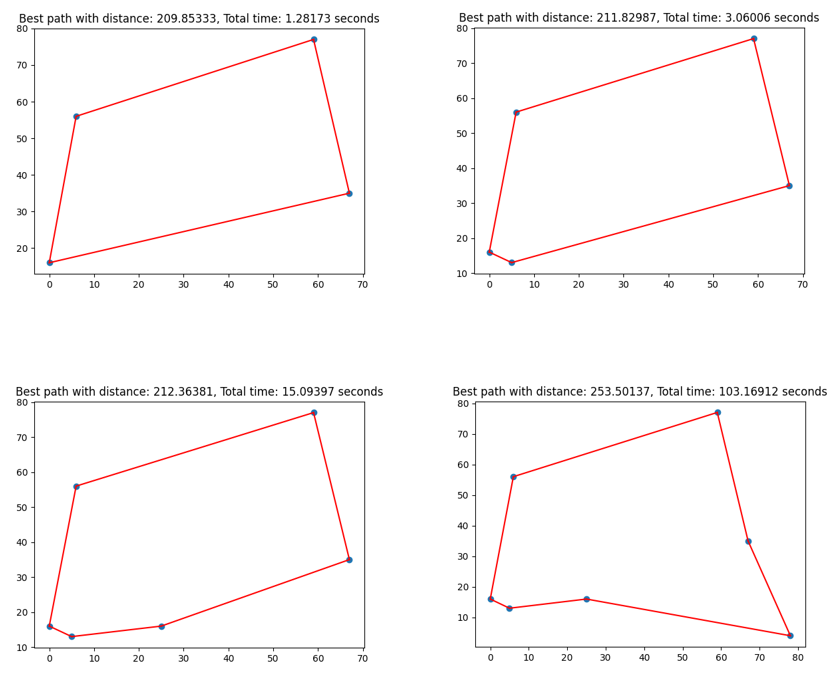
\includegraphics[width=0.8\textwidth]{
        papers/variationsprinzip_algorithmen/images/teil2/02_bruteforce_methode.png
    }
    \caption{Resultate von verschiedener Durchgänge mit steigender Anzahl von Städten}
    \label{fig:results_bruteforce}
\end{figure}

Auf dem Bild \ref{fig:results_bruteforce} ist ersichtlich, dass mit 
jedem weiteren Knoten der Aufwand exponentiell steigt. Anders 
ausgedrückt, mit jeder weiteren Stadt gibt es mehr Varianten, die 
durchprobiert werden müssen. Die Anzahl der Möglichkeiten lässt sich 
mit der Formel

\begin{equation}
    (n-1)!
\end{equation}

berechnen, wobei \(n\) die Anzahl der Städte ist.

Die Berechnung der verschiedenen Kombinationen lässt sich mit folgender 
mathematischen Formel beschreiben:

\begin{equation}
    \label{eq:bruteforce_min_formula}
    L(\sigma) = \sum_{i=1}^{n-1} d(\sigma(i), \sigma(i+1)) + d(\sigma(n), \sigma(1))
\end{equation}

Erklärung:\\
- \( L(\sigma) \)  repräsentiert die Gesamtlänge der Rundreise, die durch 
die Permutation \( \sigma \) der Städte definiert ist.\\
- \( \sigma \) ist eine Permutation der Städte \( \{1, 2, \ldots, n\} \),
wobei jedes \( \sigma \) unterschiedliche Reihenfolge der Städte darstellt.\\
- \( d(i, j) \) ist die Funktion, welche die Entfernung der Stadt \( i \) und 
Stadt \( j \) zurückgibt.\\
- \( L(\sigma) \) die Gesamtlänge der Rundreise \( \sigma \).\\

\subsection{Kurzes Beispiel Rechnung der Formel
    \label{variationsprinzip_algorithmen:section:bruteforce_calculate}}
\rhead{Kurzes Beispiel Rechnung der Formel}
Um zu verdeutlichen, wie die Formel \ref{eq:bruteforce_min_formula}
angewendet wird, folgt hier ein Beispiel.

\begin{table}[h]
    \centering
    \begin{tabular}{|c|c|c|c|c|}
        \hline
          & A  & B  & C  & D  \\ \hline
        A & 0  & 10 & 15 & 20 \\ \hline
        B & 10 & 0  & 35 & 25 \\ \hline
        C & 15 & 35 & 0  & 30 \\ \hline
        D & 20 & 25 & 30 & 0  \\ \hline
    \end{tabular}
    \caption{Beispiel Tabele mit möglicher Distanz der Städten}
    \label{tab:example_bruteforce_cities}
\end{table}

In der Tabelle \ref{tab:example_bruteforce_cities} sind die Distanzen 
zwischen den Städten A, B, C und D aufgeführt. Die Tabelle ist symmetrisch, 
da die Entfernung von Stadt A nach Stadt B gleich der Entfernung von 
Stadt B nach Stadt A ist.
Die Tabelle liesst sich wie folgt: Die Distanz zwischen Stadt B und D 25 beträgt.

Eine mögliche Permutation wäre $\sigma = (A, B, C, D)$ oder $\sigma = (B, D, A, C)$.

Setzt man die Permutation $\sigma = (B, D, A, C)$ in die Formel $\L(\sigma)$
\ref{eq:bruteforce_min_formula} ein, wird die Gesamtdistanz berechnet.


\(i\) und \(i+1\) definiert, welche Position in der Permutation betrachtet wird. 
Beispeil mit \( L(\sigma(1)) \) würde aus dem Set das B genommen und das führt 
dann zu dieser aufstellung
\begin{equation}
    L_1 = d(B, D) + d(D, A) + d(A, C) + d(C, B)
    = 25 + 20 + 15 + 35 = 95
\end{equation}
Dann werden alle möglichen Kombinationen durchgerechnet, und die kürzeste 
Strecke wird als Lösung gewählt.

\subsection{Aufwand Bruteforce
    \label{variationsprinzip_algorithmen:section:bruteforce_efforts}}
\rhead{Aufwand Bruteforce}
Aus den vorherigen Abschnitten ist ersichtlich, dass der Aufwand für die 
Berechnung der kürzesten Strecke exponentiell steigt. Mit jedem weiteren 
Knoten gibt es mehr Variationen, die durchprobiert werden müssen. 

% Tabelle
\begin{table}[ht]
    \centering
    \caption{Zeitverlauf mit steigender Anzahl von Städten}
    \begin{tabular}{cc}
        \toprule
        Punkte & Zeit       \\
        \midrule
        1      & 0,6880     \\
        2      & 0,6905     \\
        3      & 0,7666     \\
        4      & 1,2817     \\
        5      & 3,0601     \\
        6      & 15,0940    \\
        7      & 103,1691   \\
        8      & 1.068,3832 \\
        \bottomrule
    \end{tabular}
\end{table}

%TODO: find out how to make a diagram

Aus der Tabelle und dem Graphen ist ersichtlich, dass der Aufwand mit 
jeder weiteren Stadt exponentiell steigt. Mit 8 Städten dauert die
Berechnung bereits über 17 Minuten.

%%
% teil3.tex -- Beispiel-File für Teil 3
%
% (c) 2020 Prof Dr Andreas Müller, Hochschule Rapperswil
%
% !TEX root = ../../buch.tex
% !TEX encoding = UTF-8
%
\section{Teil 3
\label{000template:section:teil3}}
\rhead{Teil 3}
Sed ut perspiciatis unde omnis iste natus error sit voluptatem
accusantium doloremque laudantium, totam rem aperiam, eaque ipsa
quae ab illo inventore veritatis et quasi architecto beatae vitae
dicta sunt explicabo. Nemo enim ipsam voluptatem quia voluptas sit
aspernatur aut odit aut fugit, sed quia consequuntur magni dolores
eos qui ratione voluptatem sequi nesciunt. Neque porro quisquam
est, qui dolorem ipsum quia dolor sit amet, consectetur, adipisci
velit, sed quia non numquam eius modi tempora incidunt ut labore
et dolore magnam aliquam quaerat voluptatem. Ut enim ad minima
veniam, quis nostrum exercitationem ullam corporis suscipit laboriosam,
nisi ut aliquid ex ea commodi consequatur? Quis autem vel eum iure
reprehenderit qui in ea voluptate velit esse quam nihil molestiae
consequatur, vel illum qui dolorem eum fugiat quo voluptas nulla
pariatur?

\subsection{De finibus bonorum et malorum
\label{000template:subsection:malorum}}
At vero eos et accusamus et iusto odio dignissimos ducimus qui
blanditiis praesentium voluptatum deleniti atque corrupti quos
dolores et quas molestias excepturi sint occaecati cupiditate non
provident, similique sunt in culpa qui officia deserunt mollitia
animi, id est laborum et dolorum fuga. Et harum quidem rerum facilis
est et expedita distinctio. Nam libero tempore, cum soluta nobis
est eligendi optio cumque nihil impedit quo minus id quod maxime
placeat facere possimus, omnis voluptas assumenda est, omnis dolor
repellendus. Temporibus autem quibusdam et aut officiis debitis aut
rerum necessitatibus saepe eveniet ut et voluptates repudiandae
sint et molestiae non recusandae. Itaque earum rerum hic tenetur a
sapiente delectus, ut aut reiciendis voluptatibus maiores alias
consequatur aut perferendis doloribus asperiores repellat.





\printbibliography[heading=subbibliography]

\end{refsection}
